\chapter{Evaluation\label{cha:chapter6}}

In this chapter the implementation of the Rollup System is evaluated. The evaluation is divided into two parts: the first part evaluates the performances of the ZoKrates rollup program, while the second part evaluates the performances of the Rollup System as a whole.


% Put some screenshots in this section! Map the requirements with your proposed solution. Compare it with related work. Why is your solution better than a concurrent approach from another organization?

\section{Test Environment\label{sec:testenvir}}

ISE's department offers a server for executing the Rollup System. The server is equipped with an Intel Xeon CPU E3-1270 v6 @ 3.80GHz, 64GB DDR4 RAM, 32 GB of SWAP memory and 250GB of SSD storage. The server runs Gentoo release 2.7 Linux distribution with kernel version 5.10.52. When elsewhere specified it has been used a Google Cloud Platform virtual machine with 12 vCPU Intel Haswell, 256GB of RAM and 300 GB of SSD. This machine runs Debian 11.

The blockchain used for the Rollup System is the Tezos blockchain running on the Ghostnet testnet, with Nairobi Protocol. The rpc node used is \url{https://ghostnet.ecadinfra.com/}.


\section{Benchmarks\label{sec:benchmarks}}

\subsection{Hash Function\label{subsec:6_hashfunc}}

The hash function decision has been a key point to make the system more responsive and efficient, as the generation of the Merkle Trees and the merging process of balances and nonces rely on it. The initial programs were using sha2-256, but it was too RAM demanding and it was not possible to compile programs with more than 8 users. The implementation of the programs has been changed to use sha3-256, which revealed to be faster: ZoKrates sha2-256, in fact, adds a layer of complexity to the computation because it adds 256 bits of padding to the input, and involves more constraints in the computation. The sha3-256 implementation allowed performance increase without changing the rest of the program, as the inputs size and outputs were the same as sha2-256.
Finally the hash function has then been changed to Poseidon, which is a very zk-SNARK friendly, allowing the compilation of programs up to 1024 users. Figure \ref{fig:6_sheets-benchmarks_hash.png} shows the RAM requirements for each hash function tested compared to the amount of users and transactions.

\begin{figure}[ht]
	\centering
	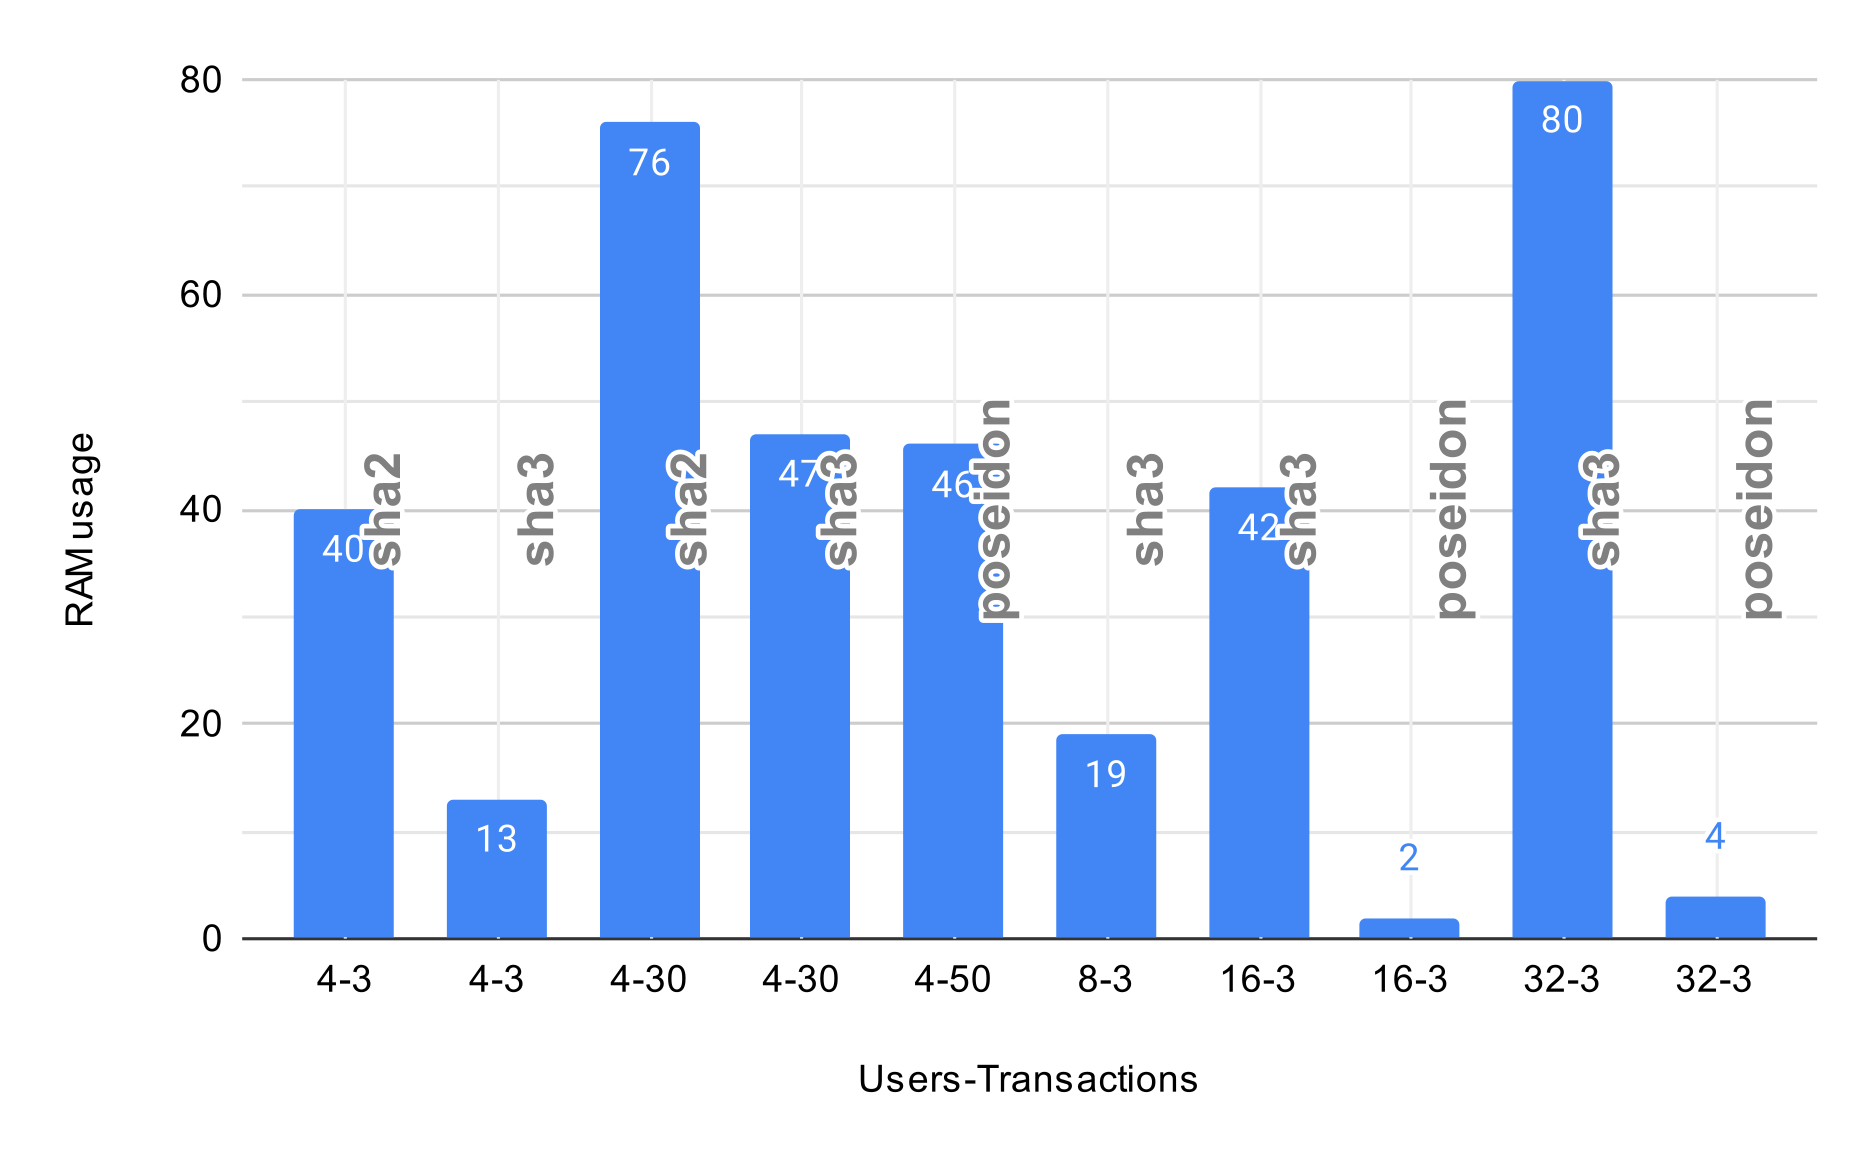
\includegraphics[width=0.7\columnwidth]{6_sheets-benchmarks_hash.png}
	\caption[RAM Usage hash]{RAM Requirements for each hash type.}  
	\label{fig:6_sheets-benchmarks_hash.png}
  \end{figure} 

\subsection{ZoKrates Rollup Performance\label{subsec:6_zokratesperf}}

A problem that emerges immediately when compiling the ZoKrates programs are the computational requirements to be able to compute the witness and generate a proof to submit to the Layer 1. The usage of the Poseidon hash function allowed the compilation of larger programs with more users and more transactions. Figure \ref{fig:6_sheets-resources-requirements.png} shows the RAM resources needed for the compilation phase of the rollup program. Note that the compilation phase is done only once, and the computation of the witness and generation of the proof are much less demanding, but those results show the complexity growth when adding transactions compared to adding users. This behavior is due to the fact that the verification of the signature still uses the sha2-256 hash function.

\begin{figure}[ht]
	\centering
	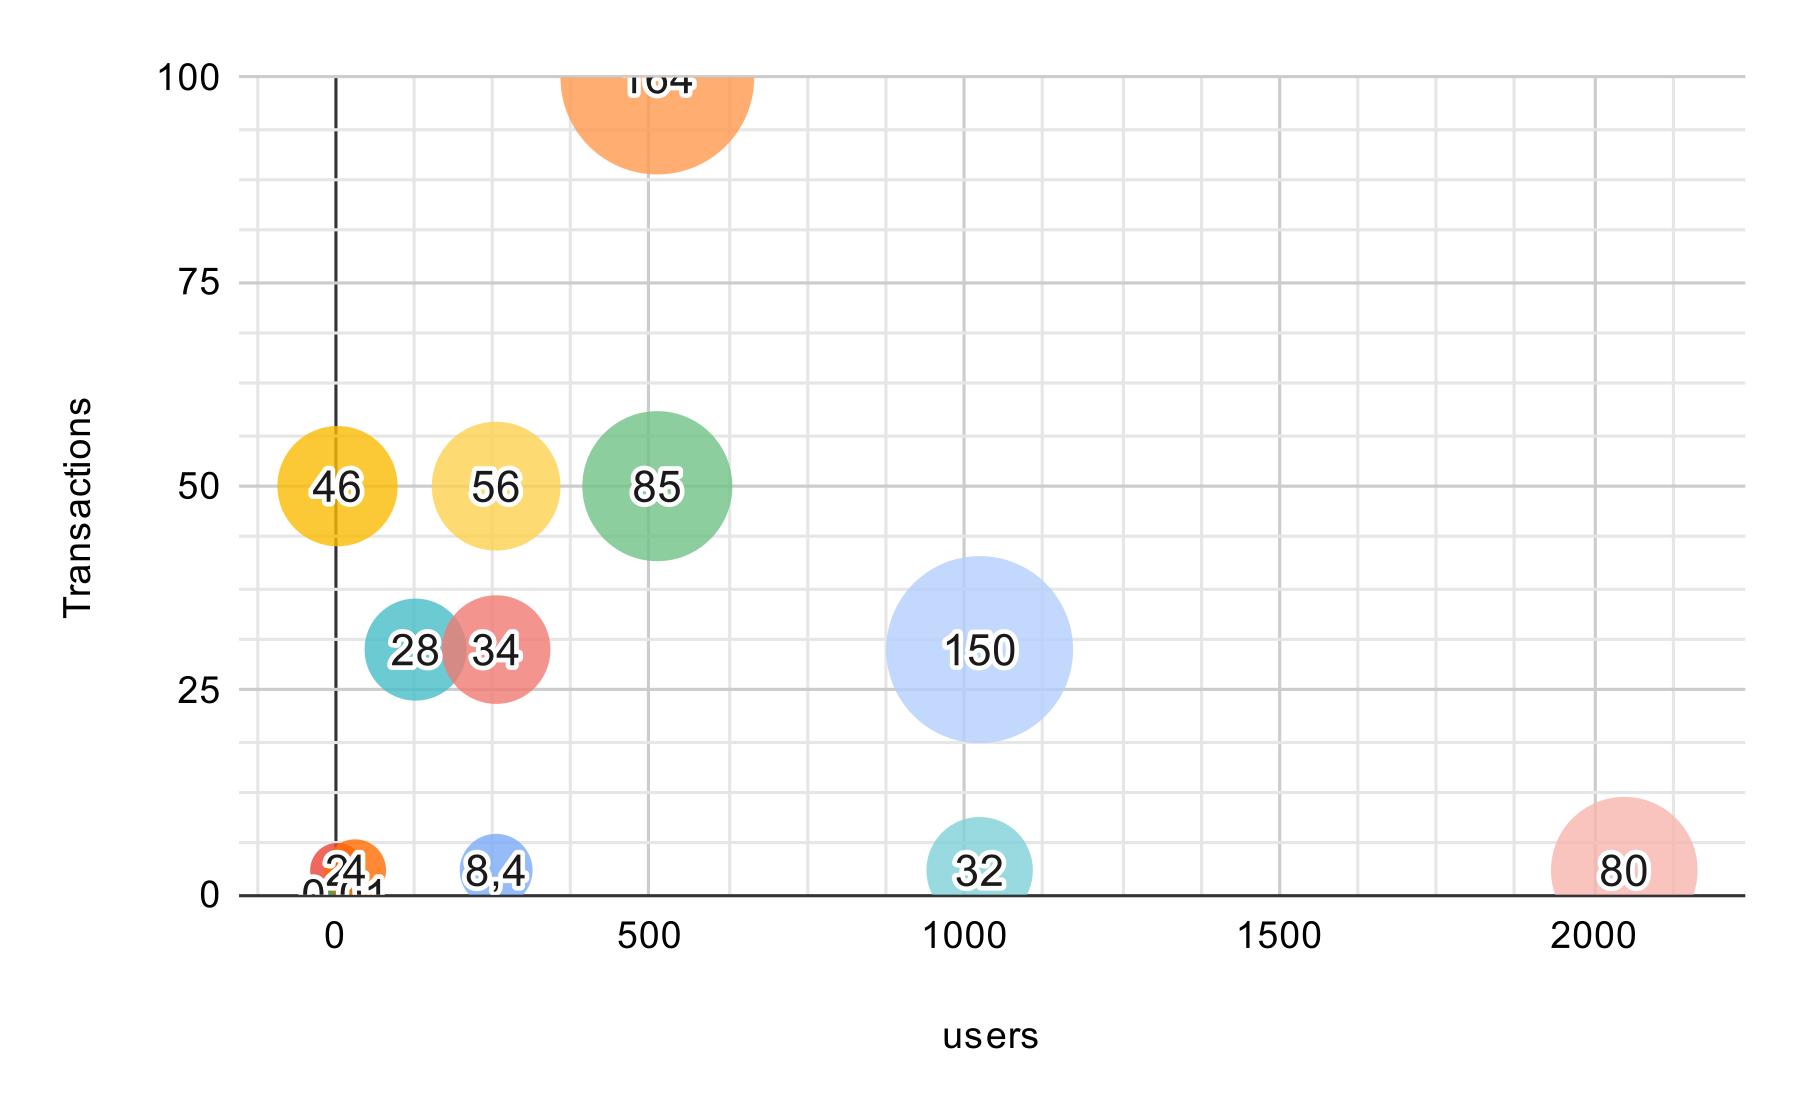
\includegraphics[width=0.7\columnwidth]{6_sheets-resources-requirements.png}
	\caption[RAM Requirements]{RAM Requirements for the compilation phase.}  
	\label{fig:6_sheets-resources-requirements.png}
  \end{figure} 

\subsection{Tezos Rollup Fees}

The verification performed by the verifier contracts and the subsequent update of the storage have costs. The verification cost is proportional to the size of the proof: during the proof verification, in fact, all the constraints are checked in a loop, consuming gas for each constraint verified. A single normal transaction between two users, as of 18/08/2023 costs 0.000518 tz.

Figure \ref{fig:6_sheets-cost-comparison.png} shows the fees for a single transaction in different scenarios of Rollup System size. The fees are calculated by submitting a rollup execution proof and looking at the fees payed for the proof verification and the storage update. The size of the bubble represent a visual amount of cost per transaction. From the graph is evident that even with a small Rollup System, the fees are very low, and they are always below the fees of a single transaction on the blockchain. Fees increase only with the increase number of transactions, due to the proof compression and reduction explained in Section \ref{sec:5_redandcompr}.

\begin{figure}[ht]
	\centering
	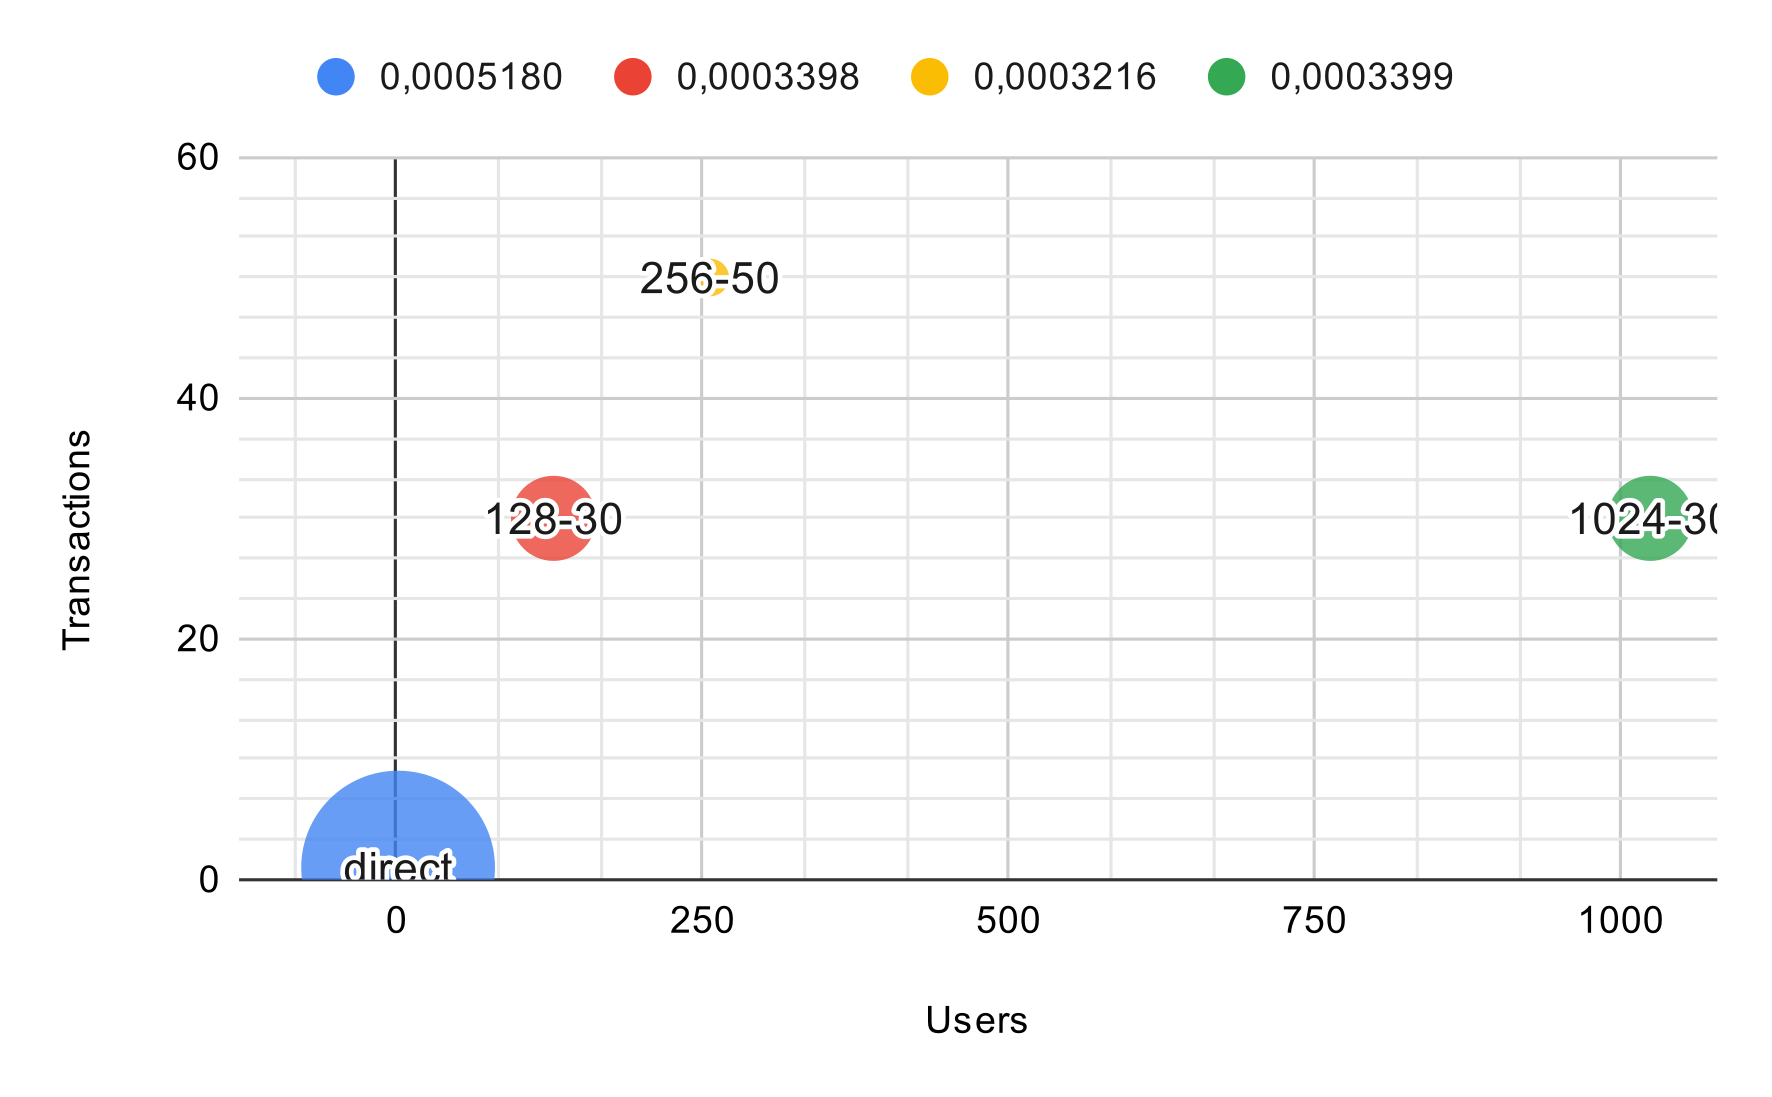
\includegraphics[width=0.7\columnwidth]{6_sheets-cost-comparison.png}
	\caption[Cost Comparison]{Cost per Transaction using different proof sizes.}  
	\label{fig:6_sheets-cost-comparison.png}
  \end{figure} 

  \section{Cost Model}

The proposed Rollup System has demonstrated greater efficiency compared to the conventional Layer 1 transaction system. However, there are additional costs that must be considered, including the expenses associated with running Layer 2 servers and the fees required for submitting and verifying proofs. In the current design, these costs are borne by the server initiating the proof. Consequently, the introduction of a fee system for Layer 2 users becomes necessary. It's important to highlight that inactive users on Layer 2 can be problematic, as they inflate the user list, thus increasing the operational costs of the entire rollup system. To address this issue, the implementation of a fee system is warranted.

\subsection{Fee System}

In order to execute a rollup, it is necessary to retrieve all users to recalculate the new Merkle root and determine the updated balances. As the number of users registering with the system increases, this process becomes slower. ZoKrates programs are capable of handling only powers of 2 numbers of users (including empty users) due to the merkle tree's structural characteristics. This can lead to exponential growth even when the number of users increases by just one.

Upon registering with the rollup system, a user transfers funds from their account to the Manager Smart Contract. This arrangement empowers the Manager Smart Contract to manage user funds by applying fees under specific circumstances. A proposed Fee Model revolves around the concept of a user's last activity, denoting the most recent instance of sending or receiving a transaction within the Rollup System. This information can be easily computed by the Manager Smart Contract while updating balances and nonces for senders and receivers after a successful proof verification.

An external server node may periodically retrieve the user list and identify stale accounts. Through a ZoKrates program that is subsequently verified, the server can compute the updated balances while levying fees on stale accounts. These fees can then be directly transferred to the Rollup Manager Smart Contract, which can utilize them to cover the costs of proof verification and storage updates.

\subsection{Reward System}

Layer 2 Rollup servers consist of two types: Web-Managers and ZoKrates executors. Web-Managers are economical servers, capable of operating with modest hardware specifications. They function as Docker containers hosting a database and node server. On the other hand, ZoKrates executors are relatively more resource-intensive, requiring a significant amount of RAM for witness computation and proof generation. However, ZoKrates executors possess an advantage: they need not run continuously, being solely necessary when computing and submitting proofs to the blockchain. This enables them to be deployed on a cloud service, activated only as needed. This approach effectively reduces the costs of Layer 2 operations while still necessitating a reward system.

Similar to the role of bakers in the Tezos blockchain when generating blocks, Layer 2 nodes can be rewarded for their contributions in submitting valid proofs. These rewards are extracted from the sender's balance during a transaction. The rewarded amounts are then attributed directly to the Rollup Manager Smart Contract's Layer 1 balance, enabling it to cover the costs of proof verification and storage updates without requiring modifications to the balance Merkle Tree.